\section{Detailed Design}
\label{sect:design}

We next present \lm in detail. Additional implementations and formalized algorithms are provided in Appendix~\ref{append:prompt_algorithm}.


\subsection{\textit{SpecAdaptation}}
We develop the core reasoning engine, \core, on top of open-source LLMs, in \textit{SpecAdaptation} to capture the cross-sentence and cross-clause relationships from the complex 3GPP specifications. To enable it to generalize and reason in 3GPP specifications, we expose \core to broad information to obtain cellular specification domain knowledge in the following two steps. 

\noindent \textbf{Cross-sentence/clause relation preserving data sanitation.} 
To ensure \core can be exposed to the broad cellular network domain knowledge, we begin by collecting and curating 5G and 4G technical specifications from the 3GPP portal~\cite{3GPP_Specs_2025} as the corpus for training. To ensure consistency and clarity, we sanitize the specifications by (a) removing redundant spaces, extraneous line breaks, and leading symbols (e.g., dots, bullets, hyphens), (b) trimming trailing punctuation, (c) discarding empty parentheses and special unicode characters, and (d) removing tables and figures, which are usually explained or demonstrated in texts. Note that \ul{references (e.g., `as specified
in subclause X.Y.Z') are preserved in the datasets}, ensuring \core can learn the cross-sentence and cross-clause relations via explicit references that are neglected by state-of-the-art works~\cite{rahman2024cellularlint}. 
 

\noindent \textbf{Domain knowledge adaptation.} A straightforward approach to expose standards knowledge to \core is to continually train (i.e., pretrain) the model on 3GPP specifications. While feasible in principle, this approach has two key limitations. 
First, pretraining a model is computationally expensive and difficult to maintain for the fast-evolving standards. 3GPP standards evolve frequently across different releases and versions. A continuously trained model can become out-of-date quickly unless training is performed repeatedly. Second, training an LLM on a narrow domain corpus (i.e., specifications) under limited compute and data diversity can degrade the model's general reasoning and instruction-following abilities~\cite{gururangan2020don, kemker2018measuring, ouyang2022training}. For example, a continually pretrained model may exhibit catastrophic forgetting and spec-confusion behaviors, such as conflating procedures across different releases, hallucinating missing steps, or recurring boilerplate in specifications. These failures are harmful for standards analysis, where correctness hinges on precise conditions, message ordering, and release-specific normative requirements.

In our design, we leverage Retrieval-Augmented Generation (RAG)~\cite{lewis2020retrieval} to adapt \core to domain knowledge without modifying the base model. Specifically, \textit{CellSec\-Inspector-Core} retrieves relevant specification excerpts and conditions its generation on them, using the retrieved text as grounded evidence to complement its parametric knowledge. 
The retrieval corpus is organized as versioned specification chunks, where each chunk preserves the source specification number, release/version, clause identifier, and cross-reference information.
Concretely, given a query (e.g., message type, timer, or a security requirement), it searches a versioned corpus of 3GPP documents, which is prepared in the aforementioned step, and attaches the top-matched paragraphs (including section and release/version identifiers) to the model prompt. This retrieval step provides two technical benefits: (i) it ensures that \core uses the explicitly selected release/version text, and (ii) it reduces hallucination by requiring outputs to be justified by retrieved normative statements rather than relying solely on the model’s memory. Finally, \core obtains the 3GPP specification domain knowledge, and it will be further used in all modules. The detailed workflow is provided in Algorithm~\ref{alg:rag_prompt} in Appendix~\ref{append:prompt_algorithm}.


\subsection{\textit{SCA Representation Extractor}}
\label{subsect:sca_representation}

To address C1 and comprehensively model the complicated cellular network functions, we develop the \textit{SCA (State-Condition-Action) Representation Extractor} that extracts the structured function representations in SCA nodes from 3GPP specifications. Each SCA node contains four fields: the start state, representing the initial state before the transition; the condition, denoting the triggering clause or prerequisite specified in the text; the action, describing the operation mandated by the specification upon satisfaction of the condition; and the end state, indicating the resulting state after the action is executed. 

\noindent\textbf{SCA node vs. FSM state.} Different from the traditional finite state machine (FSM) that separates the states and transitions and stores the transition logic on edges between states, the SCA representation structure (i.e., node) aims to directly capture the self-contained transition, binding the logic of condition and action. This structure introduces two main advancements to maximize the utilization of the text processing capability of \core. 
First, it presents explicit transition semantics, including where the transition starts, when it is valid (condition), what happens (action), and where it ends. Each SCA node is one self-contained transition. 
The explicit viewpoint of a transition saves the step of merging all involved edges in the FSM when transitioning from one state to another.  
That is, an FSM state may have several edges with its connected states, requiring extra effort to identify how to transition to the next state. 
Second, it allows complex conditions and actions, combining internal variables, timers, and status, to be described in a single node, which is valuable for modeling cellular network functions where the transitions may depend on complicated conditions and actions. \textit{Note that SCA nodes can be easily transformed into the FSM states and edges. However, it is challenging to transform them in reverse.} 


\noindent\textbf{Few-shot training with minimal dataset development overhead.}  
To extract SCA nodes from 3GPP specifications, instead of developing a large dataset of many SCA nodes training cases with heavy manual engineering overhead, we leverage efficient in-context learning (ICL)~\cite{brown2020language} to educate \lm without time-consuming fine-tuning to update model parameters.
ICL works by embedding carefully selected demonstration examples and task-specific instructions directly into the model’s input context, allowing the model to infer the desired output format. This method enables \lm to generalize to the SCA extraction task with a limited number of examples. 
Specifically, we instruct \lm to extract structured specification events from 5G and 4G specifications by mapping each relevant sentence into an SCA node. 
Along with the instruction, a few manually developed SCA nodes are given for \lm to infer. From each specification, we develop two examples to demonstrate common specification patterns. 
Sentences that accurately describe function events are expected to populate all four fields. 
If a sentence contains cross-references (e.g., `as specified in subclause X.Y.Z'), the referenced content is retained verbatim in the most relevant field. For ambiguous or underspecified sentences, we employ best-effort inference. If no definition is found, the corresponding field is marked as `Not explicitly defined' to ensure completeness of the extracted structure. Figure~\ref{fig:sca_extractor_prompt} in Appendix~\ref{append:prompt_algorithm} shows an example ICL instruction. 


\begin{figure}[t]
  \centering
  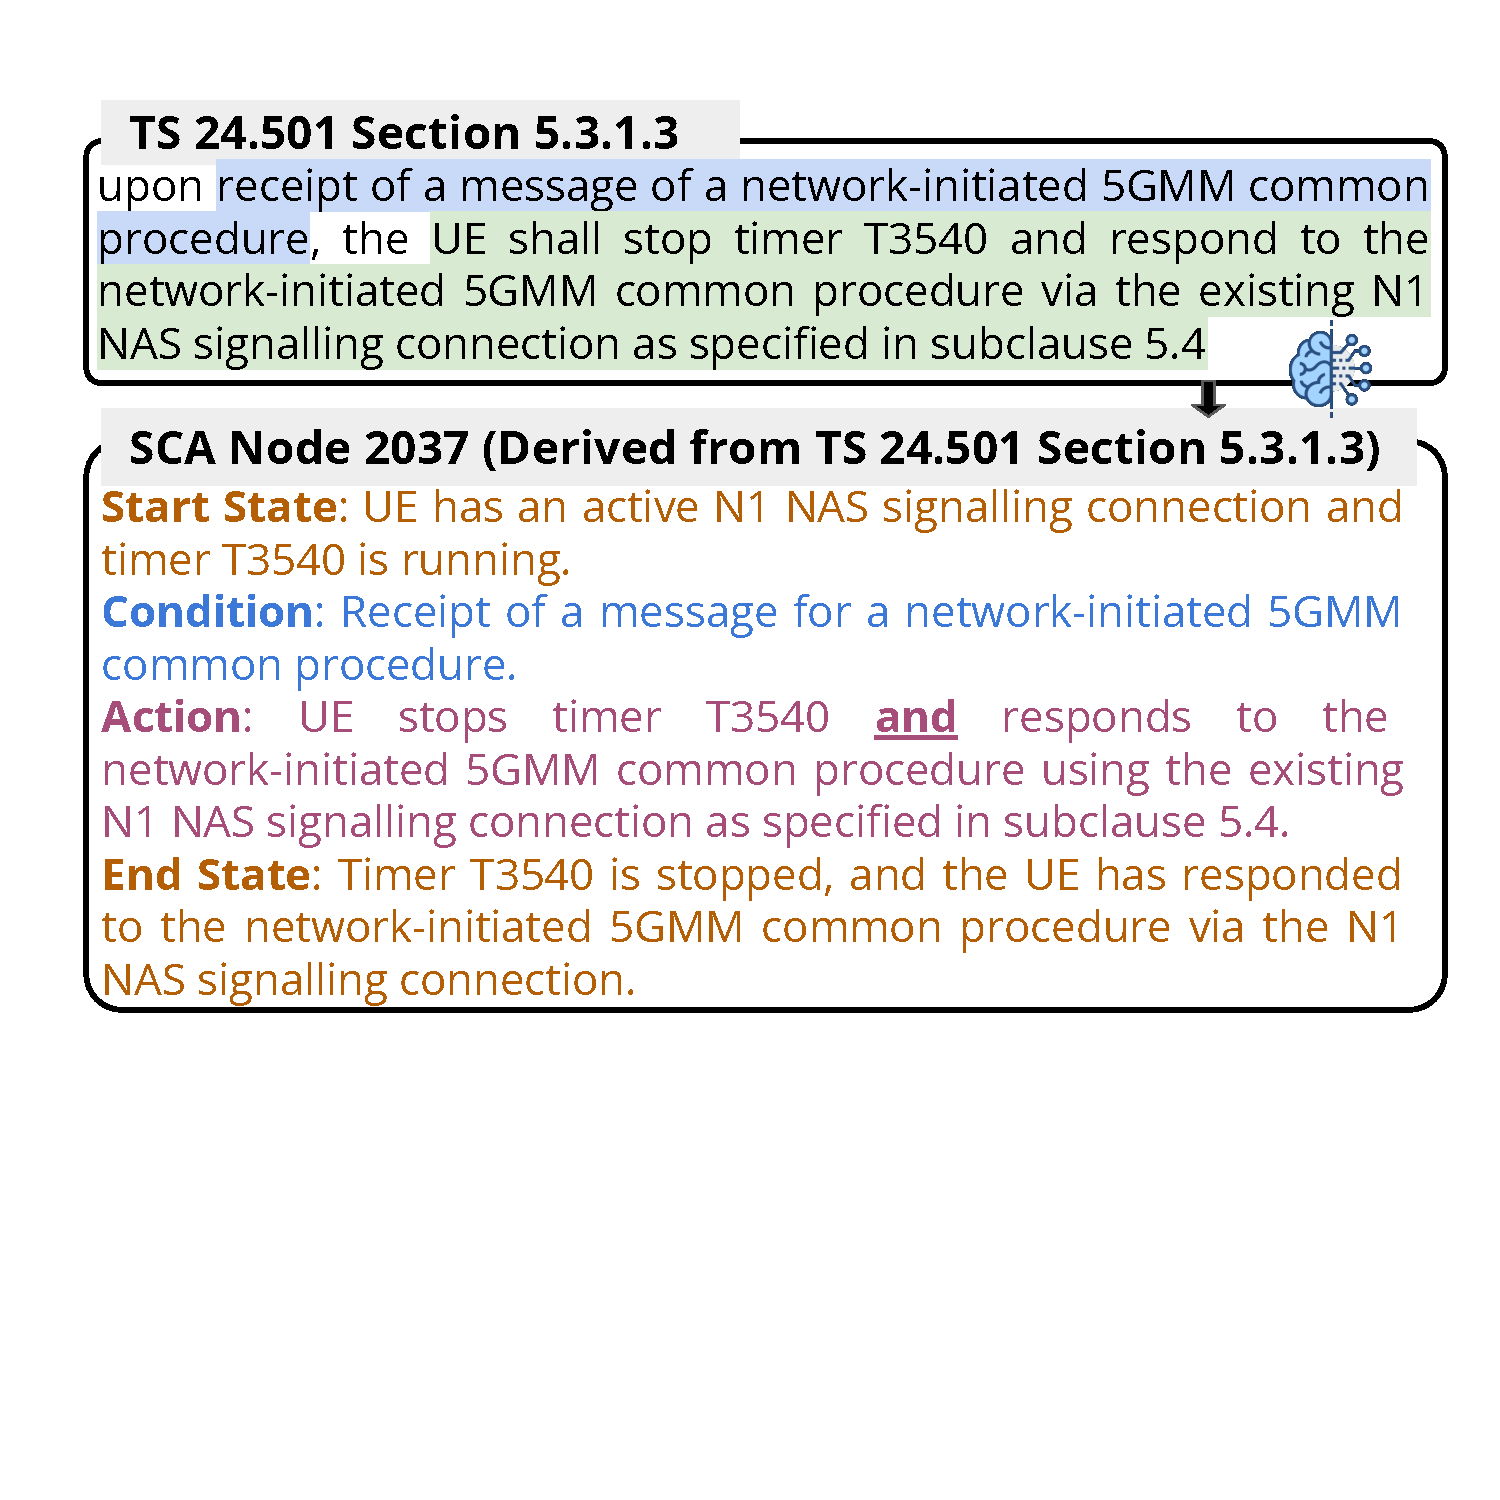
\includegraphics[width=0.85\linewidth]{pic/SCA-node-v1.pdf}
  \vspace{-0.1in}
  \caption{SCA representation for Node 2037}
  \label{fig:SCAnode} 
  \vspace{-0.2in}
\end{figure}

\noindent\textbf{SCA node example.} 
Figure~\ref{fig:SCAnode} presents an extracted SCA node from a short description in 5G NAS specification TS 24.501 by the following steps.       
\lm first parses the sentence structure using domain knowledge learned in \textit{SpecAdaptation}. There was no explicit start state in this given example. \lm identifies the triggering condition by detecting the phrase upon receipt of a message, recognizing that the transition is activated when the UE receives a message for a network-initiated 5GMM common procedure. Next, \lm extracts the actions from the phrases `\textit{shall stop timer T3540}' and `\textit{respond to the procedure},' which are organized as the structured expression that covers these two operations: stop T3540 \textbf{and} respond via the existing N1 NAS signalling connection as specified in subclause 5.4. From the derived condition and action, including `\textit{via the existing N1 NAS signalling connection}' and `\textit{timer T3540}', it is inferred that the UE already maintains an active N1 NAS signalling connection and T3540 is running before the event occurs, which are captured as the start state. Last, \lm derives the end state according to the start state, condition, and actions: after stopping T3540 and responding, the UE remains connected via the N1 NAS signalling connection, but T3540 is no longer running. In a traditional FSM, it is impractical to infer the start and end states, and two operations in the action may bring unnecessary difficulties in determining which edges shall be included within complicated FSM transitions when there are thousands of connected states.  



\subsection{\textit{Function Chain Builder}}
After extracting scattered SCA nodes, each representing a self-contained state transition, we assemble them into coherent function chains, which complete the transitions for representing the complex mobile network functions specified in 3GPP specifications. Notably, this task is non-trivial due to the challenge outlined in \textbf{C2} (Section~\ref{subsect:challenges}), where thousands or more SCA nodes can be developed from thousands of pages from a single 3GPP specification. To construct complete function chains from these scattered SCA nodes, two types of connection strategies are designed: 


\subsubsection{Type I: Node-Informed Exhaustive Connection}
~This category uses exhaustive pairwise comparisons between SCA nodes to discover all valid transitions. Three connection methodologies are defined:


\noindent \textbf{(a) Temporal Connection.} 
A temporal connection captures the most basic dependency between SCA nodes. It identifies whether the end state of an SCA node is identical to the start state of another. Formally, let the set of extracted SCA nodes be $N = \{n_1, n_2, \ldots, n_m \}$, where each node $n_i$ is defined as   
\[
n_i = (\text{start}(n_i), \text{condition}(n_i), \text{action}(n_i), \text{end}(n_i)).
\]
\noindent Each node $n_i \in N$ is associated with a start state and an end state that $\text{start}(n_i), \; \text{end}(n_i) \in Q$, where $Q$ denotes the set of all specification states extracted from the 5G and 4G NAS and RRC specifications. 
The Temporal-Connection relation \( T \) is defined as 
\(T = \{ (n_i, n_j) \in N \times N \mid \text{end}(n_i) = \text{start}(n_j) \} \). 
SCA node \(n_j\) is a valid temporal successor of \(n_i\) if the start state of \(n_j\) is identical to the end state of \(n_i\). 
The formalized algorithm is shown in Algorithm~\ref{alg:temporal_connection} in Appendix~\ref{append:prompt_algorithm}.
As shown in Figure~\ref{fig:eventchain}, the SCA Node 2110 extracted from the 5G NAS specification presents a transition from 5GMM-IDLE mode with suspend indication to 5GMM-CONNECTED mode upon receiving an indication from lower layers that the RRC connection has resumed. Another Node 2055 represents a transition starting exactly in 5GMM-CONNECTED mode, describing the transition from 5GMM-CONNECTED to 5GMM-CONNECTED with RRC inactive. Because the end state of Node 2110 is identical to the start state of Node 2055, they meet the requirement for a valid temporal connection. 

\noindent \textbf{(b) \textbf{Semantic Connection.}} Temporal Connection requires that two SCA nodes must have exactly the same end state and start state. However, 3GPP specifications are written by different experts. There may be slight differences in textual descriptions for the identical concepts or functions in 3GPP specifications, which we refer to as \textit{textually different but semantically equivalent descriptions}.
To connect SCA nodes with such a relation, we introduce Semantic Connection, which identifies if the end state \(\text{end}(n_i)\) of Node $n_i$ and the start state \(\text{start}(n_j)\) of Node $n_j$ are semantically equivalent or strongly related. If so, Node $n_j$ is allowed to be the successor of Node $n_i$, even when the textual descriptions of \(\text{end}(n_i)\) and \(\text{start}(n_j)\) differ. Formally, given two SCA nodes, we check whether their semantics are $sem(\text{end}(n_i),\ \text{start}(n_j)) = \text{Yes}$ 
to associate the SCA nodes with \textit{textual descriptions different but semantically equivalent} for their end states and start states. In our approach, we leverage \core, which has been trained with extensive domain knowledge, to compare their semantic meaning. It takes 3 steps: (i) the SCA nodes' start and end states are tokenized; (ii) the transformer layers are used to build contextual embeddings based on tokens; (iii) the embeddings are further compared via cosine similarity and enhanced verification via ICL to distinguish deeper logic relations, such as entailment, contradictions, and overlaps. 
This relation \( S \)
is defined as
\[
S = \left\{(n_i, n_j) \in N \times N \;\middle|\; sem(\text{end}(n_i),\ \text{start}(n_j)) = \text{Yes} \right\} 
\]
The formalized algorithm is illustrated in Algorithm~\ref{alg:semantic_connection} in Appendix~\ref{append:prompt_algorithm}.
As shown in Figure~\ref{fig:eventchain}, Node 5263 ends in a state where the UE is in 5GMM-IDLE mode and has initiated the registration procedure due to a change in its radio capability.  
Node 2107 begins in a state where the UE is attempting to send a REGISTRATION REQUEST message. 
It proceeds to enter 5GMM-IDLE mode and continues the registration procedure. Although the end and start states are described differently, they both refer to the same specification state, the UE initiating a registration procedure triggered by updated radio capability. This represents a valid semantic connection. 

\begin{figure}
    \centering
    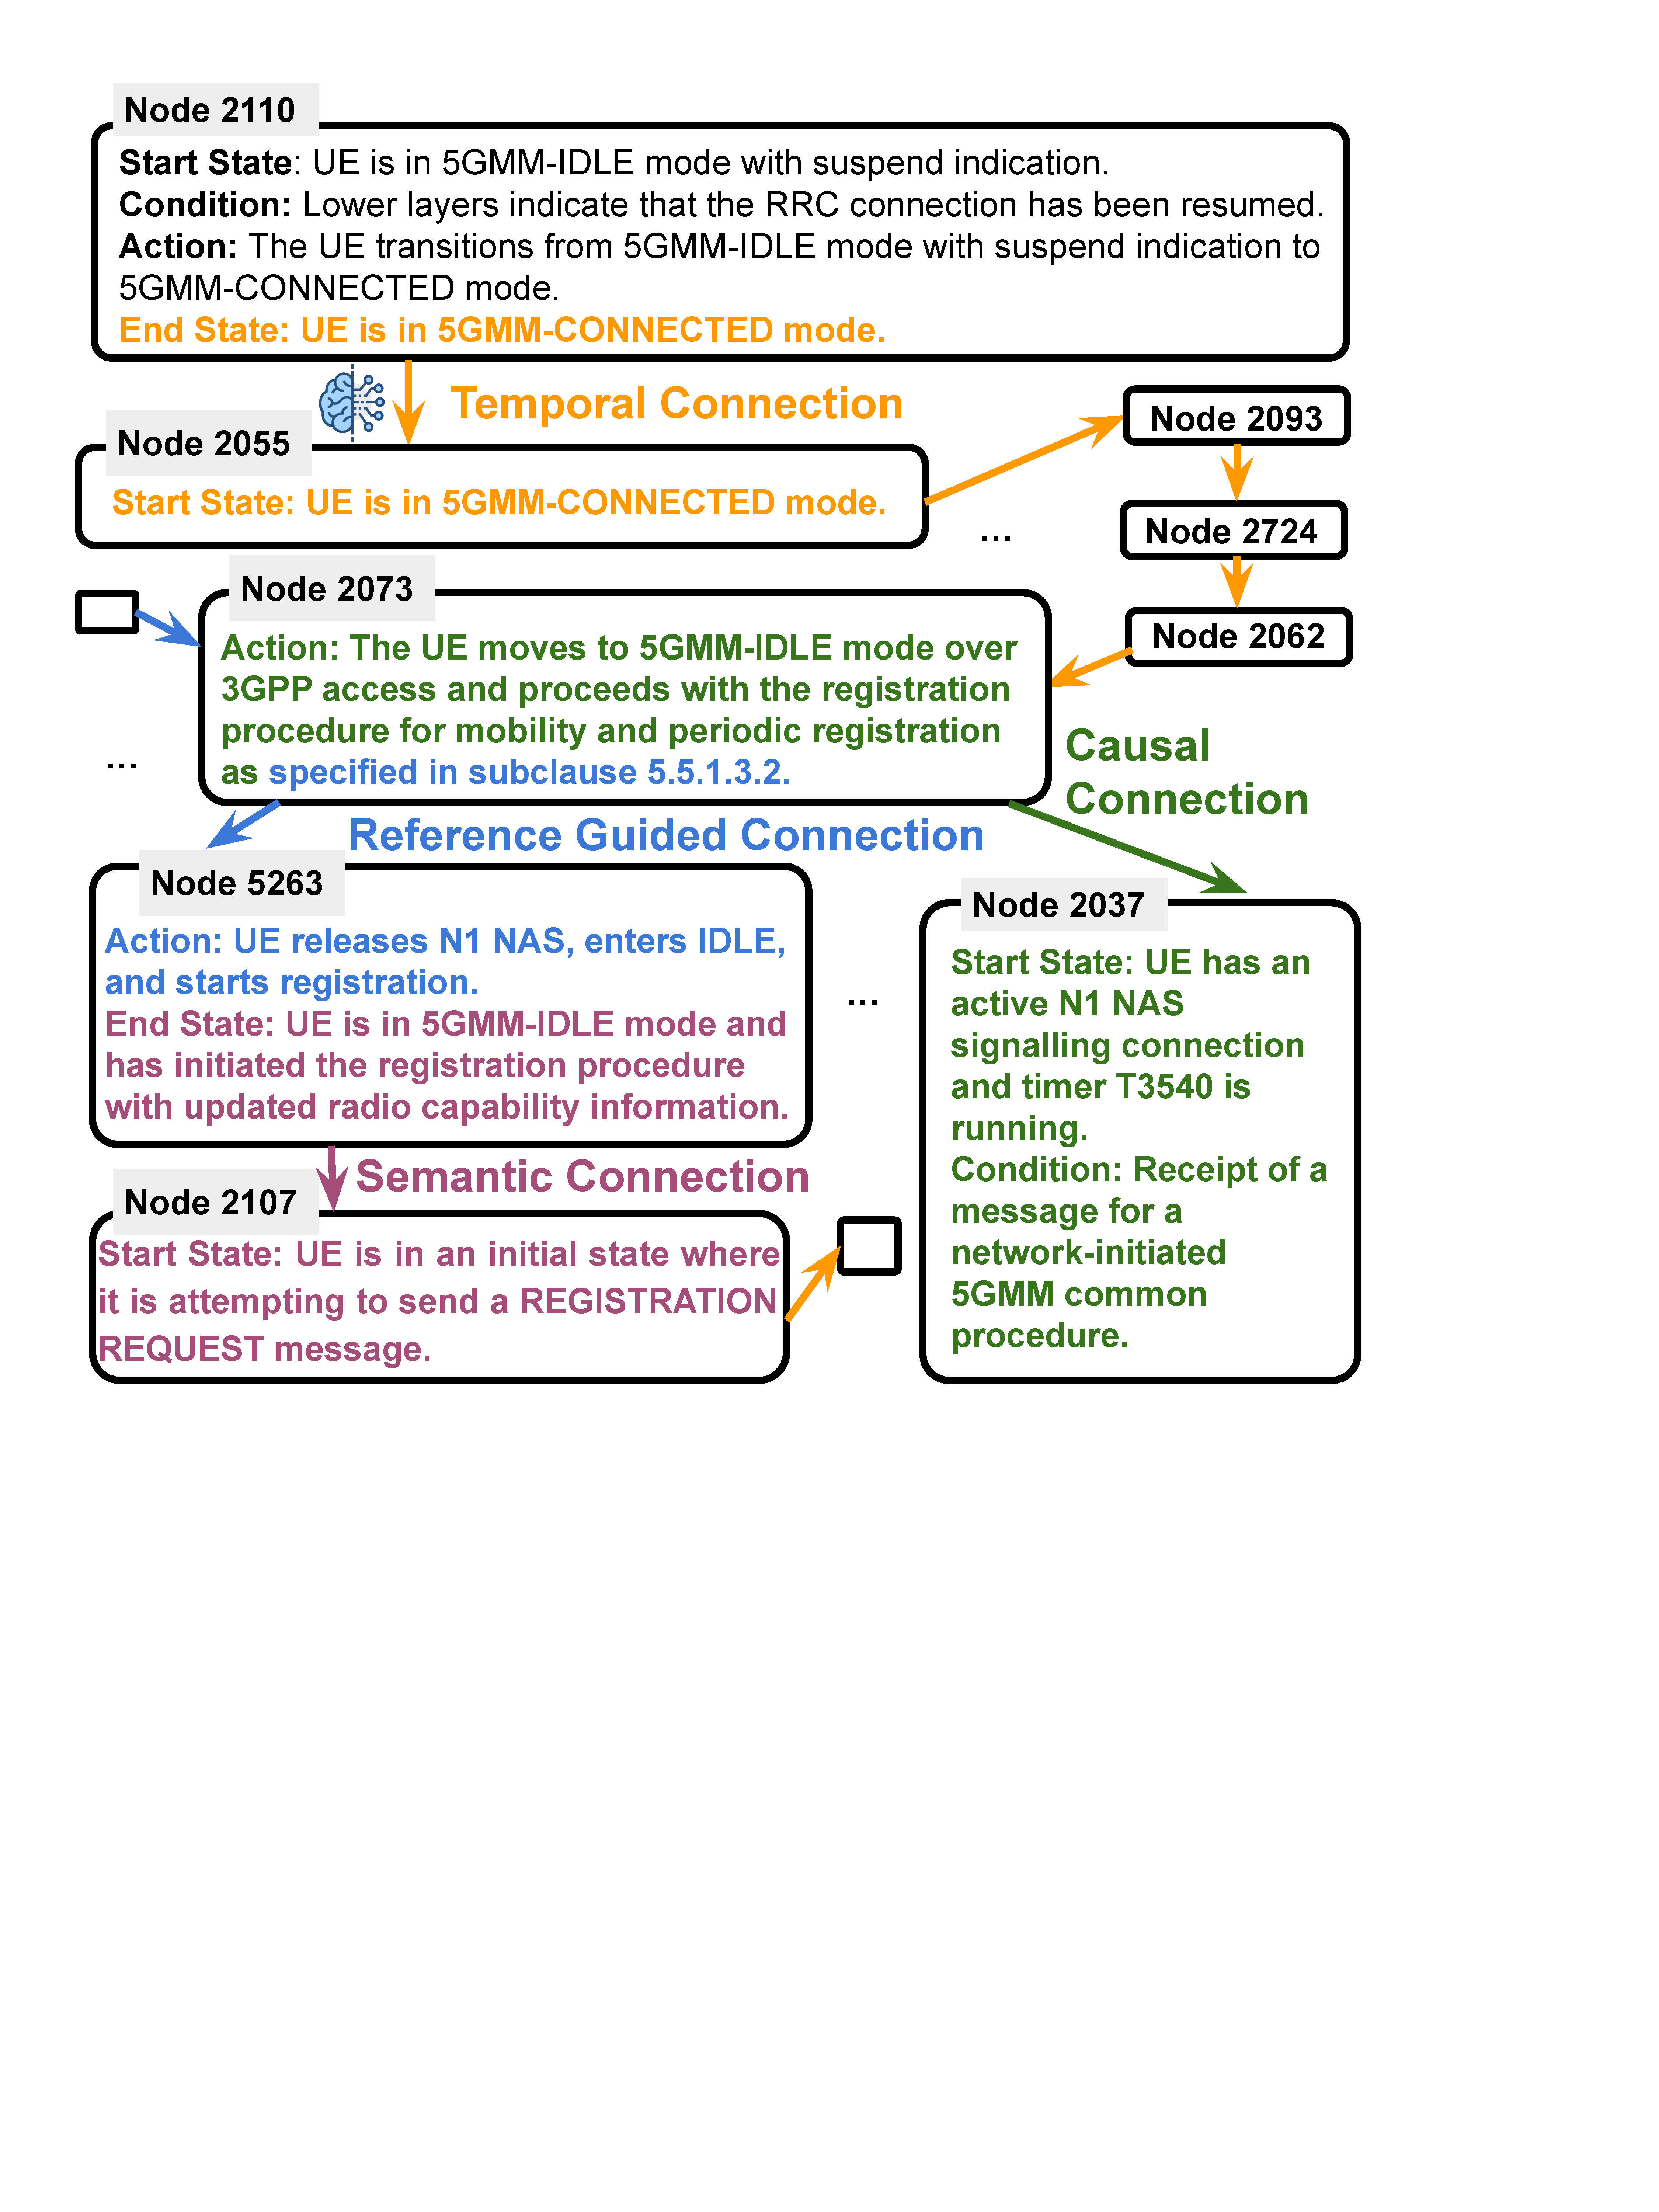
\includegraphics[width=0.86\linewidth]{pic/Function_Chain.pdf}
    \vspace{-0.1in}
    \caption{5G mobility management function chain}
    \label{fig:eventchain}
    \vspace{-0.1in}
\end{figure}

\noindent \textbf{(c) \textbf{Causal Connection.}}
Beyond the direct matching of end and start states, function chains can be causally constructed through causal relationships, where the states, conditions, or actions of one SCA node directly enable, influence, or trigger the states, conditions, or actions of another.  
That is, the states, conditions, or actions in $n_i$ serve as a plausible prerequisite or cause for the states, conditions, or actions in $n_j$, suggesting a likely sequential or dependent relationship. 
Identifying causal connections between nodes is essential to thoroughly construct complete and coherent function chains. 
We define this Causal-Connection relation $C$ such that for any pair of SCA nodes $(n_i, n_j)$, a connection exists if $ C = \{ (n_i, n_j) \in N \times N \, |\ \begin{array}{l}
\text{causal}(n_i, n_j) = \text{Yes}
\end{array}
\}$. 
The formalized algorithm is shown in Algorithm~\ref{alg:causal_connection} in Appendix~\ref{append:prompt_algorithm}.
\core is employed to infer such causal relations. 
It analyzes SCA nodes $n_i$ and $n_j$ and determines whether $n_i$ precedes $n_j$. For example, if the end state of $n_i$ transitions the UE into a mode that is required as the start state of $n_j$, or if the condition in $n_i$ (e.g., radio capability change) leads to a logically subsequent condition in $n_j$ (e.g., registration request trigger), or if the action in $n_i$ (e.g., releasing NAS signaling connection) sets up the environment necessary for the action in $n_j$ (e.g., initiating a new signaling procedure), a causal relationship is inferred.


As shown in Figure~\ref{fig:eventchain}, Node 2073 models the UE transitioning from 5GMM-CONNECTED to 5GMM-IDLE mode and initiating a registration procedure. As part of this process, the UE establishes an N1 NAS signalling connection, which is necessary for subsequent communication with the network. 
Node 2037 begins in a state where such a signalling connection is already active and the UE is ready to handle network-initiated 5GMM common procedures. 
Its condition, receiving a message from the network, relies on the existence of an active signaling context. 
This requirement is fulfilled by the action in Node 2073, which creates the signaling connection through registration. With this context, Node 2037 can further proceed to receive or respond to the network-initiated procedure. 
Therefore, the action in Node 2073 is a prerequisite for the state and condition of Node 2037. We identify it as a valid causal connection $(n_{2073}, n_{2037}) \in C$.  

\subsubsection{Type II: Reference Guided Connection} 
~While the connection strategies in Type I can, in principle, be applied to all SCA nodes, this approach is computationally expensive as discussed in \textbf{C3} (see Section~\ref{subsect:challenges}).  
A single 3GPP specification can yield thousands of nodes, and across the more than 2,000 specifications that define operational 5G and 4G mobile networks~\cite{3gppspecs}, exhaustive pairwise validation is infeasible. 
To reduce the computational cost, we constrain the search space so that each SCA node is only checked with other nodes within the same subclause. However, this restriction risks constructing incomplete function chains. 
We introduce the Reference Guided Connection to address it. 
To ensure consistency and maintainability, 3GPP specifications are written in a highly modular style, relying heavily on cross-references to avoid redundancy and to coordinate contributions across multiple working groups. 
These references are the key to Reference Guided Connection, which works as follows: 
\noindent \textbf{1. Reference Detection}: Identify whether an SCA node \( n_i \) contains references to specific clauses (e.g., `\textit{as specified in subclause X.Y.Z}'). 
\textbf{2. Space Expansion}: Extract the referenced clause and retrieve all candidate nodes \( n_j \) within that clause. 
\textbf{3. Connection Validation}: Apply Type I connections to determine if a valid connection exists between \( n_i \) and \( n_j \).
The formalized algorithm is shown in Algorithm~\ref{alg:reference_connection} in Appendix~\ref{append:prompt_algorithm}.

As illustrated in Figure \ref{fig:eventchain}, we apply the Reference Guided Connection strategy to link Node 2073 and Node 5263. First, Node 2073 explicitly cites subclause 5.5.1.3.2 in its action field, which specifies the registration procedure triggered by radio capability updates. Based on this reference, all SCA nodes derived from subclause 5.5 are considered candidate targets, including Node 5263.
We then apply Type I mechanisms to validate whether a true dependency exists. In this instance, a Causal Connection from Node 2073 to Node 5263 is detected. Specifically, Node 2073 initiates a registration procedure. This behavior corresponds to the more detailed process described in Node 5263, where the registration is triggered by a radio capability change. The action in Node 2073 logically precedes and leads to the action in Node 5263, whose execution realizes the registration behavior initiated in Node 2073. Although their start and end states differ, the procedural flow from Node 2073 to Node 5263 is a causal dependency. Thus, it is a valid Reference Guided Connection.


\subsubsection{Complete Function Chain}~Applying all proposed connection strategies to analyze the relations among SCA nodes, the \textit{Function Chain Builder} can efficiently and comprehensively construct the function chain. 
These function chains serve as structured models of complex mobile network services. Figure~\ref{fig:eventchain} depicts the constructed function chains that model 5G mobility management.   

\subsection{SecOracle}
\label{subsect:secoracle}

\textit{SecOracle} (\ul{Sec}urity \ul{Oracle}) is an adaptive security validation module to assess the security of procedures and functions defined in 3GPP specifications. Current methods, such as exhaustive character-altered testing (i.e., random fuzzing~\cite{godefroid2020fuzzing}), manually developing mobile network procedure-specific requirements~\cite{chen2023sherlock,al2024hermes}, or manually translating FSM models into SMV language~\cite{clarke1996symbolic,al2024hermes,hussain20195greasoner,hussain2018lteinspector}, are inefficient and unscalable for assessing large-scale function chains (\textbf{C2} in Section~\ref{subsect:challenges}). 

To address this, we propose a two-step approach: 
First, we define a set of security properties, which are different from the security requirements in prior works that are specific to each procedure or FSM model~\cite{chen2023sherlock,al2024hermes}. \ul{These properties encapsulate the fundamental requirements for entire mobile networks, encompassing both mobile users and network infrastructure operators.} They thus can cover a wider range of scenarios and conditions. 
Derived from security standards (e.g., 3GPP Security Assurance Methodology (SECAM)~\cite{3gppTR33916v16}, ITU-T X.805~\cite{ituTX805}) and classic security models (e.g., Dolev-Yao~\cite{dolev2003security}, Bell-LaPadula~\cite{lapadula1996secure}, and Biba Models~\cite{Biba}), we build 9 core security properties in total (see Appendix~\ref{append:securityproperties}) to cover key security dimensions. The followings are a partial of our defined security properties: \texttt{authentication}, ensuring only legitimate users or entities can initiate procedures; \texttt{authorization}, enforcing that state transitions, such as NAS transitions, are exclusively triggered by legitimate, authenticated entities; \texttt{service integrity and confidentiality}, requiring all communications to be properly secured, with mobile entities verifying message integrity and confidentiality to prevent adversaries from launching attacks such as MitM. 

Second, motivated by the fact that cellular network devices, including UEs, base stations, and function modules in Core Network, do message exchanges all the time, 
4 fundamental attack methods, including dropping, modifying, injecting, and replaying, denoted as $A$ are applied to each node and node transition. \textit{SecOracle} leverages its reasoning capability to systematically analyze whether function chains still meet all security properties under these 4 attacks. Formally, given $\forall R_i \in $Security Properties, $\forall n_j \in \text{C}$ for each function chain, $\forall a_k \in \text{A}$,  the security property verification is expressed as, 
\(
\text{CheckViolation}(R_i, n_j, a_k).
\)
A candidate violation is flagged and recorded as 
\(
C, a_k, n_j \models \neg R_i
\) 
for further analysis. 
Figure~\ref{fig:secoracle} in Appendix~\ref{append:prompt_algorithm} shows how \core is instructed in this module.

\noindent \textbf{From candidate violations to confirmed vulnerabilities.}  
\textit{SecOracle} outputs candidate violations rather than confirmed vulnerabilities. Both candidate violations and confirmed vulnerabilities refer to \textit{design defects} in 3GPP specifications. A candidate violation indicates that a function chain may violate a security property under an adversarial action and therefore requires further validation. We classify a candidate as a confirmed vulnerability only if it satisfies three criteria: (i) the flagged violation is grounded in the corresponding 3GPP specifications; (ii) the issue reflects a specification-level design weakness rather than only an implementation-specific behavior; and (iii) the issue can lead to a realistic security consequence, such as unauthorized state transition, service disruption, privacy leakage, or inconsistent UE/network state. 
 

\noindent \textbf{Violation example.} Consider the function chains shown in Figure~\ref{fig:eventchain}. For each node, \textit{SecOracle} applies 4 attack methods to assess possible candidate violations against security properties. In Node 2073, the UE sends a REGISTRATION REQUEST to transition from 5GMM-CONNECTED to 5GMM-IDLE mode. As a detected candidate violation shown in Figure~\ref{fig:output_secoracle}, under a replay attack, if this REGISTRATION REQUEST is intercepted and replayed, the network may process it again. According to 3GPP 5G NAS specification TS 24.501 subclause 4.4.4.3~\cite{3GPP_TS_24501}, the AMF must accept such a message even if it is unauthenticated and lacks integrity protection. 
The acceptance of an unauthenticated initial REGISTRATION REQUEST is a bootstrapping mechanism in a zero-trust environment. However, as reported in GSMA CVD\#0029~\cite{hussain20195greasoner}, the AMF may disconnect an existing legitimate UE connection after receiving an unauthenticated initial REGISTRATION REQUEST, before the requesting entity has been sufficiently authenticated or verified. In this case, the attacker can exploit the fact that an unauthenticated request can trigger security-sensitive connection-state changes. These inconsistencies can lead to billing errors, misrouted downlink traffic, or even session management failures. In severe cases, adversaries can repeatedly force the UE to re-register, thereby disrupting ongoing sessions and achieving a denial-of-service (DoS) attack using forged NAS messages. This is a specification design vulnerability; the violated property is \texttt{service integrity}: security-sensitive actions, such as releasing an existing UE connection or replacing an active UE context, should not be triggered solely by an unauthenticated message before sufficient verification. 


\begin{figure}[t]
\centering
\begin{minipage}{0.98\columnwidth}
\begin{lstlisting}[style=myjsonblock]
| 2062 | 2073 | Replay | BEGIN_JSON {
  "vulnerability_detected": "Yes",
  "violated_property": [5],
  "explanation": "A Replay attack could exploit the transition from 5GMM-CONNECTED mode with RRC inactive indication to 5GMM-IDLE mode by capturing and retransmitting the REGISTRATION REQUEST message. This violates the Replay Attack Protection requirement.",
  "test_case": "An attacker captures the REGISTRATION REQUEST message during the transition and retransmits it, causing the AMF to process the same message twice, leading to potential registration failures or security breaches.",
  "vulnerability_source": "event2073"
} END_JSON |
\end{lstlisting}
\end{minipage}
\vspace{-0.1in}
\caption{A candidate violation flagged by \textit{SecOracle} for Nodes 2062 and 2073 transition}
\label{fig:output_secoracle}
\vspace{-0.1in}
\end{figure}


\subsection{VulnTestGenerator}

After detecting 
candidate violations by \textit{SecOracle}, \textit{VulnTestGenerator} generates corresponding testing procedures for validating whether these candidates can be confirmed as vulnerabilities.  
It aims to narrow the gap between specification-level findings and real-world verifications. As shown in Figure~\ref{fig:vulnTestGenerator} in Appendix~\ref{append:prompt_algorithm}, \textit{VulnTestGenerator} is instructed via ICL to develop structured test cases that specify network states, security context status, UE and core network configurations, operation sequences, and expected outputs, from flagged candidate violations. Those test cases can guide us how to validate and observe the violated security properties. 
Table \ref{tab:replay-2073} in Appendix~\ref{append:testcase} presents an example test case for validating the security property \texttt{service integrity} violation in Node 2073,  
which describes a specific behavior in TS~24.501 Subclause~5.3.1.4, where a UE in 5GMM-CONNECTED mode with RRC inactive indication sends a REGISTRATION REQUEST with the NG-RAN-RCU bit set for UE radio capability update and then moves to 5GMM-IDLE.


\noindent \textbf{Validating violations with test cases.} Executing the generated test cases on either a controlled testbed (e.g., open5GS~\cite{open5gs}, srsRAN-\ ~\cite{srsran}) or an operational mobile network allows us to validate the vulnerability and find the root cause. Notably, conducting real-world experiments requires substantial human effort, including building experimental platforms, instrumenting the network/UE to collect experimental data, and analyzing results. The current scope of \textit{VulnTestGenerator} focuses on generating test cases to guide these validation experiments. Executing test cases in an automated manner is a non-trivial activity. We leave it as future work.     



